\chapter{Approach 2: L-System Music Generation}

One of the biggest challenges in producing music from accounts is simply that we're using a small amount of simple data (amounts of money) to derive music, which is far more complex (sequences of notes, cords, etc). To meet this challenge, an approach is needed in which we can encourage music to ``emerge'' from something as simple as a company's balance sheet. To this end, we will turn to the field of \textbf{Biologically-Inspired Computing}.

Biologically inspired techniques tend to be good for solving complex problems with no obvious solution. Applying these techniques often leads to emergent properties, which is exactly what we're looking for. One such technique is that of the \textbf{L-System}.

In this chapter, we will look at using L-Systems to generate music from accounts. Two possible variations to achieving this will be looked at, with the most promising approach chosen for implementation and evaluation. With a working implementation, we will perform a preliminary evaluation, and then experiment with the rule generation.

\section{Definitions}

\begin{center}
\begin{singlespace}
\begin{tabular}{ l l }
\hline
\hline
\textbf{L-System}: & A Biologically-Inspired parallel re-writing system. \\ \hline
\textbf{Grammar}: & Set of symbols unique to a specific L-System. \\ \hline
\textbf{Rules}: & Part of an L-System. Specifies re-writing strategies. \\ \hline
\textbf{Axiom}: & A string of characters on which an L-System operates. \\ \hline
\hline
\end{tabular}
\end{singlespace}
\end{center}

\section{An Introduction to L-Systems}

\textbf{L-Systems} (also known as Lindenmayer Systems) were developed in 1968 by Aristid Lindenmayer. Lindenmayer was a biologist, who was trying to understand the behaviour of plant cells. During the process of his research, he developed the idea of ``an axiomatic theory of biological development''\footnote{\url{http://www.biologie.uni-hamburg.de/b-online/e28_3/lsys.html}}, which became known as the L-System. Nowadays, L-Systems have applications ranging from modeling the physical structure of plants to computer graphics. They can also be used to generate music.

L-Systems allow the re-writing of a string of characters based on a set of rules. An L-System has a \textbf{grammar}, \textbf{rules} and a \textbf{start axiom}. An L-System $G$ is formally defined as follows:

\begin{singlespace}
\begin{formality}
$G = \{ V, S, \omega, P \}$
\end{formality}
\end{singlespace}

$V$ is a set of \textbf{variables} (replaceable symbols), and $S$ is a set of \textbf{constants} (non-replaceable symbols). $P$ are the \textbf{re-writing rules} of the L-System, and $\omega$ is the \textbf{start axiom}. Rules given in $P$ will be applied to $\omega$ each time the L-System is run. 

A common example of an L-System in action is one which generates the \textbf{Fibonacci Sequence}. The Fibonacci Sequence is a sequence of numbers with very special properties. The first Fibonacci number is always 0, and the second Fibonacci number is always 1. After that, each subsequent number is defined as the sum of its two predecessors. Below is the definition of this L-System:

\begin{singlespace}
\begin{formality}
$V = \{ A, B \}$ \\
$S = \{\}$ \\
$\omega = \langle A \rangle$ \\
$P = \{ (A \rightarrow B), (B \rightarrow AB) \}$
\end{formality}
\end{singlespace}

Each time we run this L-System, we work through all the symbols in $\omega$, turning each `A'  into a `B', and each `B' into an `AB'. If we count the length of the axiom $\omega$, we get the next number in the Fibonacci Sequence:

\begin{singlespace}
\begin{formality}
start: A (axiom length = 1)\\
1st run : B (axiom length = 1)\\
2nd run : AB (axiom length = 2)\\
3rd run : BAB (axiom length = 3)\\
4th run : ABBAB (axiom length = 5)\\
5th run : BABABBAB (axiom length = 8)\\
6th run : ABBABBABABBAB (axiom length = 13)
\end{formality}
\end{singlespace}

From these simple rules, we witness a more complex property emerging. But, what happens if we define our grammar as something that can be interpreted musically?

\section{Design}
Recall that with the \textbf{Signal Mapping}, we derived signals from an account. These signals represented changes. We mapped then these signals directly to musical sequences. This time, we will instead use these signals to drive an L-System to generate music.

Two options are open for consideration. One option, is to use the accounts to generate the \textit{rules} of the L-System. The alternative is to use the accounts to generate the \textit{starting axiom}, and apply a manually crafted set of rules. Let's consider the merits of these two approaches.

\section{Variation 1: Dynamic Rule Generation}

If we decide to use the account to generate the rules, we are having to generate both the variables and the constants. Therefore, the process of generating the rules from the account must consider both musical structure (the constants in $S$) and reduction strategies (the variables in $V$). As we are generating music, we should therefore attempt to hold as much control over the constant symbols of $S$ as possible, as it is these elements that will directly translate into music.

We could be more efficient by simply using the accounts to generate the variable symbols, and define the constant symbols ourselves so that they conform to musical structures. In doing so, we may as well separate the constants and variables from one another, placing these variables in the start axiom. Doing this has the added advantage of resulting in a dynamic start axiom that will be unique for each account.

By this logic, we can conclude that Dynamic Rule Generation is \textit{not} the most efficient approach to use. But, by simplifying this idea we have derived a better approach; that of \textbf{Dynamic Axiom Generation}.

\section{Variation 2: Dynamic Axiom Generation}
Recall that instead of generating the rules from the accounts, we have chosen to manually define the rules to conform to sensible musical sequences. This way we can be assured that the L-System will produce musical sequences that will conform to what we understand to be \textit{music} rather than a chaotic collection of notes.

Now, consider that we now use the accounts to directly generate the start axiom. This will result in a unique axiom for each account, which when operated on by the L-System will produce an equally unique piece of music. The question then becomes, how can we use data in the account to generate an appropriate starting axiom?

The signal generation from the \textit{Signal Mapping} implementation presents us with a way of evaluating the health of an account, and we can build on this idea with an L-System. We can divide the potential spread of signal values into discrete grades (remember that a signal strength above \textit{1.0} indicates an increase, and below \textit{1.0} indicates a decrease). For example, let's say we try a six grade system:

\begin{singlespace}
\begin{formality}
$A > 1.25$\\
$1.25 \geq B > 1.15$\\
$1.15 \geq C > 1.05$\\
$1.05 \geq D > 0.95$\\
$0.95 \geq E > 0.85$\\
$F \leq 0.85$
\end{formality}
\end{singlespace}

By doing this, we map signal ranges to symbols. If we include these characters in the grammar of our L-System as replaceable symbols, we can define the set of variables $V$ as:

\begin{singlespace}
\begin{formality}
$V = \{ A, B, C, D, E, F \}$
\end{formality}
\end{singlespace}

\noindent An arbitrary account may therefore result in the following starting axiom\footnote{Note that although usually L-Systems uses a string to represent its axiom, I have chosen to use a \textbf{list} of \textbf{characters}. In the implementation, we will see that a list is easier to manipulate in Python.}:

\begin{singlespace}
\begin{formality}
$\omega = \langle C, D, A, B, B \rangle$
\end{formality}
\end{singlespace}

At this stage, we have successfully defined two parts of an L-System: The set $V$ of variables, and we can derive the start axiom $\omega$ from an account. The next step is to carefully choose a set of symbols which can be interpreted as music. These symbols will form the constants of $S$ in our L-System. It is at this stage that we need to decide on an appropriate grammar.

\section{Defining a Grammar}

If we look at music from the point of view of how a note in a sequence relates to its predecessor, then a note can be in one of three states; higher, lower or unchanged. We can use this to begin defining the set of variables $V$.

\begin{singlespace}
\begin{formality}
Let `u' = raise note by a tone\\
Let `d' = lower note by a tone\\
Let `s' = sustain note
\end{formality}
\end{singlespace}

Given a starting note, from these three symbols we can generate a sequence of notes. However, this grammar is quite limited, and we would like to expand it so it can better represent many more musical aspects such as chords, and key changes. To this end, we can expand the grammar with the following additions:

\begin{singlespace}
\begin{formality}
Let `/' = Raise note by two tones\\
Let `\_' = Lower note by two tones\\
Let `r' = Don't play anything (rest)\\
Let `.' = Increase overall key by a semi-tone\\
Let `,' = Decrease overall key by a semi-tone\\
Let `j' = Shift into a major key\\
Let `n' = Shift into a minor key
\end{formality}
\end{singlespace}

It would also be nice to add a harmony to complement a melody (a harmony in this case is a note played $n$ semi-tones above the note of the melody):

\begin{singlespace}
\begin{formality}
Let `+' = Turn on harmony\\
Let `-' = Turn off harmony
\end{formality}
\end{singlespace}

With this, we have a full grammar for the set $S$ of variables:

\begin{singlespace}
\begin{formality}
$S = \{ $`u', `d', `s', `/', `\_', `r', `.', `,', `j', `n' $\}$
\end{formality}
\end{singlespace}

\section{Adding Stacks to the Grammar}

In computer science, a \textbf{stack} is a primitive (yet invaluable) data structure which only allows items to be added and removed from its top. Therefore the fist item into the stack will be the last item removed, and vice-versa.

Why would we need to make use of stacks in \textit{this} L-System? Without a mechanism to jump back to earlier points in the sequence, the music would meander up and down, with no specific points to break it up. Adding a stack brings more musical structure, and allows different account attributes to affect parts of the music independently.

Many L-System implementations have built in support for the use of stacks. So, when we play the music from an axiom produced by this L-System, if we encounter a stack ``push'' symbol  (which looks like `\textbf{[}'), the program will record the current note, chord and key signature. It then continues playing the music until it reaches a stack ``pop'' symbol (which looks like `\textbf{]}'). When this happens, the program resets the note, chord and key signature to its earlier state, and continues playing the axiom.

\begin{singlespace}
\begin{formality}
Let `[' = Push current state onto stack\\
Let `]' = Pop current state from stack
\end{formality}
\end{singlespace}

\section{Interpreting the Grammar}

Turning the grammar in the axiom into music is a simple matter. Let $note$ be the current note, $tonic$ be the tonic (root note of the current key) and $scale$ be the scale (major or minor) of the current key. Let $harmony$ be whether a harmony note is being played or not.

\begin{singlespace}
\begin{formality}
$note \rightarrow \{ 21 \leq note \leq 108, note \in \mathbbm{N} \}$ \\
$tonic \rightarrow \{ 21 \leq harmony \leq 108, harmony \in \mathbbm{N} \}$ \\
$scale \rightarrow \{ major, minor \}$ \\
$harmony \rightarrow \{ true, false \}$
\end{formality}
\end{singlespace}

We initialise $note$, $tonic$, $scale$ and $harmony$ to values of our choosing, and begin to process the axiom into \textit{MIDI} values. Chords are calculated by playing a triad from the current key (notes 1, 3 and 5 of the scale)


\section{An Example in Action}

Let's look at a simple parsing example. Consider the following axiom $\omega$ generated by our L-System after a few runs:

\begin{singlespace}
\begin{formality}
$\omega = \langle$ `s', `u', `u', `d', `[', `u', `u', `u', `u', `]', `s', `d', `d', `d' $\rangle$
\end{formality}
\end{singlespace}

If we set our starting note to Middle C (MIDI value of 48), the above would transcribe the following sequence of notes:

\begin{singlespace}
\begin{formality}
48, 50, 52, 50, 52, 54, 56, 58, 50, 48, 46, 44
\end{formality}
\end{singlespace}

\section{Selecting the Rules}

With the axiom being generated by the account, the rules of the L-System must be defined manually. As we want our generated sequences to sound as musical as possible, we should ensure that our rules define short sequences with proper musical structure. To do this, we enforce some constraints when defining these short sequences.

To begin with, we can choose a \textbf{time signature}. Doing so means that we should have a consistent amount of notes in each sequence. For example, a time signature of 4 beats per bar would mean that the number of notes in each sequence must be divisible by 4.

So, we as a result of this, we might define the rules for our six-grade system as follows:

\begin{singlespace}
\begin{formality}
$( A \rightarrow j..uuuu )$\\
$( B \rightarrow [..suud] )$\\
$( C \rightarrow uuu\_uuu\_ )$\\
$( D \rightarrow ddd/ddd/ )$\\
$( E \rightarrow [,,sddu] )$\\
$( F \rightarrow n,,dddd )$
\end{formality}
\end{singlespace}

This defines some suitable musical sequences, which are appropriate for the account signal ranges they're representing. However, you will notice that after one iteration of the L-System, the axiom will be fully reduced (ie, will consist entirely of non-replaceable symbols).

To complete the rule set, we need to keep producing replaceable symbols at each iteration.  This might be done by modifying the rules to appear as follows:

\begin{singlespace}
\begin{formality}
$( A \rightarrow j..uuuuB )$\\
$( B \rightarrow [..suud]D )$\\
$( C \rightarrow uuu\_uuu\_A )$\\
$( D \rightarrow ddd/ddd/F )$\\
$( E \rightarrow [,,sddu]C )$\\
$( F \rightarrow n,,ddddE )$
\end{formality}
\end{singlespace}

The way in which the L-System produces music is often surprising, and it is not immediately obvious how to place the variables within the rules. On one hand, we want to have the music mimic the account as closely as possible. On the other hand, we want to encourage the emergence of interesting music from the L-System.

To help us choose which replaceable symbols to use, I propose that we can visualise members of $V$ occurring in $P$ as a \textbf{Finite State Machine} (FSM). In this way, when we define the set of rules $P$, we can see how the L-System will reduce the axiom $\omega$ \textit{(figure \ref{fig:fsm1})}.

\begin{figure}[ht]
\centering
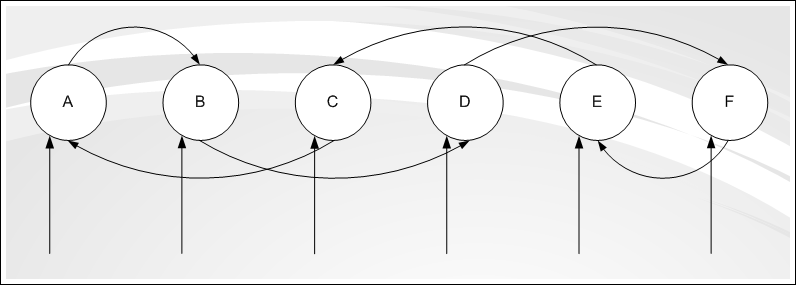
\includegraphics[scale=1.5]{fsm1}
\caption{A Finite State Machine showing a possible application of replaceable symbols within the rules of an L-System.}
\label{fig:fsm1}
\end{figure}

From \textit{figure \ref{fig:fsm1}}, we can see that our rules are probably not all that sensible. For example, $A$ reduces to a string containing $D$. This leads to more varied music being generated, but prevents a true impression being given of an account. A more sensible strategy is given in the \textit{figure \ref{fig:fsm2}}.

\begin{figure}[ht]
\centering
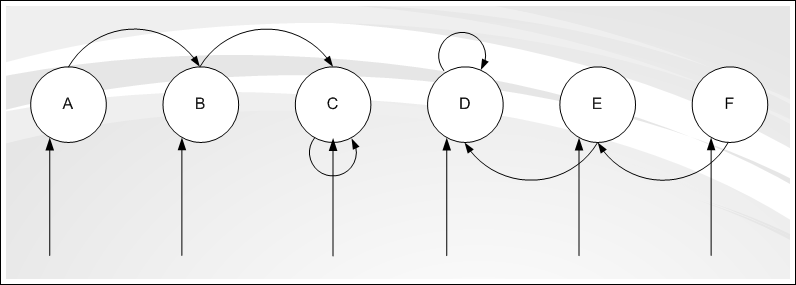
\includegraphics[scale=1.5]{fsm2}
\caption{A Finite State Machine showing a more sensible application of replaceable symbols within the rules of an L-System.}
\label{fig:fsm2}
\end{figure}

This gives us the following rules:

\begin{singlespace}
\begin{formality}
$( A \rightarrow j..uuuuB )$\\
$( B \rightarrow [..suud]C )$\\
$( C \rightarrow uuu\_uuu\_C )$\\
$( D \rightarrow ddd/ddd/D )$\\
$( E \rightarrow [,,sddu]D )$\\
$( F \rightarrow n,,ddddE )$
\end{formality}
\end{singlespace}


\section{Selecting the Number of Iterations}

With all parts of the L-System now defined, there remains one important question: How many iterations should the L-System run for?

To help answer this question, we might choose to think about the overall length of the final piece of music. If we can make a decision on roughly how many beats in total the music should play for, then we can arrange the program to keep running the L-System until the axiom length meets this requirement.

There is a good reason for taking this approach. As the listener will be paying close attention to the music, they may suffer from listening fatigue\footnote{Listening Fatigue is a lapse in concentration caused when the brain has to work hard to interpret what it's hearing. During the evaluation, testers will have to listen to lots of these musical sequences. Therefore, listening fatigue is a real concern.}, so the music should not play for too long.


\section{Programming Functions for an L-System}
The first step of implementation is to program a set of functions which can represent an L-System. By keeping as close to the formal definition as possible, and by making use of \textit{Python}'s lists and tuples, we define the following functions:

\begin{singlespace}
\begin{formality}
\texttt{getLSystem( V, S, w, P )}: Takes in the elements of an L-System, and validates them to ensure that the L-System is properly defined. If it is, it returns a tuple representing the L-System. If not, it returns an empty tuple. \\\\
\texttt{runLSystem( lSystem )}: Takes in a valid L-System tuple and applies the rules against the start axiom. It then returns the modified L-System tuple.\\\\
\texttt{getAxiom( lSystem )}: Takes in an L-System tuple, and extracts the axiom, returning it as a list of elements.
\end{formality}
\end{singlespace}

Recall that it is common for many L-Systems to make use of stacks. Therefore, this implementation implicitly includes the stack operators ``['' and ``]'' in the set of constants.

The L-System functions are kept separate from the rest of the L-System implementation, and reside in a function library \texttt{Linden.py}, which is imported into the main implementation.

\section{Programming the Axiom Generator}
The bulk of the implementation for the L-System generator resides in a new function library called \texttt{LSS.py}. Once again, we import \texttt{Settings.py} (which contains all the settings) and \texttt{Shared.py} (which contains functions shared across implementations).

For the most part, the implementation directly mimics the design strategy discussed so far in this chapter. We will begin by looking at the part of the program which generates the start axiom. Consider the following functions:

\begin{singlespace}
\begin{formality}
\texttt{generateAxiomSixGrade( signals )}: Returns a start axiom generated by splitting signal ranges into six grades.\\\\
\texttt{generateAxiomTenGrade( signals )}: Returns a start axiom generated by splitting signal ranges into ten grades.
\end{formality}
\end{singlespace}

For example, we feed the function \texttt{generateAxiomSixGrade()} the following signal list: \texttt{[1.513267626990144, 1.4732345248474281, 0.6928702010968921, 0.6676837725381415, 1.4555288461538463]}. The axiom returned might be: \texttt{['A', 'A', 'F', 'F', 'A']}. (The values which specify the grade boundaries are declared in \texttt{Settings.py}).

\section{Programming the Axiom Parser}

Interpreting the final axiom generated by the L-System is more involved than generating the start axiom. Given that we have a melody, a harmony and chords (chords are made up of \textit{three} notes), this gives us a total of \textbf{five concurrent note sequences} which are generated from the axiom. To this end, we represent each note sequence as a list of MIDI values (integers), and these lists are returned in a tuple of order 5.

The following functions are used when parsing the axiom, and are called depending on the nature of the current symbol (note that variables of set $V$ in the axiom are simply ignored during parsing):

\begin{singlespace}
\begin{formality}
\texttt{appendHarmony( outputMusicHarmony, currentNote, harmonize, harmonyKey, keyMap )}: Takes in a list of harmony notes (\texttt{outputHarmony}) and uses the other parameters to append the harmony note to this list. It then returns it.\\\\
\texttt{getDefaultKeyMap( keyMap )}: Returns a \texttt{keyMap} which is used by functions such as \texttt{pitchUp()} to determine where adjacent notes are in the scale.\\\\
\texttt{pitchUp( note, keyMap )}: Increases \texttt{note} to the next note above in the scale.\\\\
\texttt{pitchDown( note, keyMap )}: Decreases \texttt{note} to the next note below in the scale.\\\\
\texttt{doublePitchUp( note, keyMap )}: Increases \texttt{note} two note up in the scale.\\\\
\texttt{doublePitchDown( note, keyMap )}: Decreases \texttt{note} two note up in the scale.\\\\
\texttt{keyShiftUp( keyMap, shiftDistance, note )}: Shifts \texttt{keyMap} up by \texttt{shiftDistance}. Returns a shifted \texttt{keyMap} and a shifted \texttt{note} as a pair.\\\\
\texttt{keyShiftDown( keyMap, shiftDistance, note )}: Shifts \texttt{keyMap} down by \texttt{shiftDistance}. Returns a shifted \texttt{keyMap} and a shifted \texttt{note} as a pair.\\\\
\texttt{getChord( keyMap )}: Returns a tuple consisting of the 1st, 3rd and 5th note of the scale.\\\\
\texttt{chordComparison( currentChord, lastChord )}: Compares two chords. If the two chords are the same, it sustains the chord. Otehrwise, it plays the new chord. This is used to stop the chord being re-played each beat.\\\\
\texttt{keySwitchMinor( keyMap )}: Shifts \texttt{keyMap} into a minor key.\\\\
\texttt{keySwitchMajor( keyMap )}: Shifts \texttt{keyMap} into a major key.
\end{formality}
\end{singlespace}

\noindent With these functions now written and successfully tested for robustness, we have two more functions to define which complete the program:

\begin{singlespace}
\begin{formality}
\texttt{produceMusic( axiom, startNote, keyMap )}: Takes in an axiom, a start note and a key signature. Returns a tuple with lists of MIDI values.\\\\
\texttt{main( argv )}: The main() function which is invoked when the program is run. It reads the accounts, generates and runs the L-System, calls \texttt{produceMusic()} and then outputs the music.
\end{formality}
\end{singlespace}

As these two functions are so important, their pseudocode is given below. Firstly we'll look at \texttt{produceMusic()}:

\begin{singlespace}
\begin{formality}
\begin{itemize}
	\item[\textbullet] \texttt{produceMusic( axiom, startNote, keyMap ):}
	\begin{itemize}
		\item[\textbullet] \texttt{Initialise currentNote = startNote}
		\item[\textbullet] \texttt{Initialise currentChord = NULL}
		\item[\textbullet] \texttt{Initialise outputMusic = $\langle$$\rangle$}
		\item[\textbullet] \texttt{Initialise harmony = NULL}
		\item[\textbullet] \texttt{Initialise harmonize = false}
		\item[\textbullet] \texttt{Initialise noteStack = $\langle$$\rangle$}
		\item[\textbullet] \texttt{For each character in axiom:}
		\begin{itemize}
			\item[\textbullet] \texttt{if $c$ == `u' then increase currentNote by 1 tone}
			\item[\textbullet] \texttt{if $c$ == `d' then decrease currentNote by 1 tone}
			\item[\textbullet] \texttt{if $c$ == `/' then increase currentNote by 2 tones}
			\item[\textbullet] \texttt{if $c$ == `\_' then decrease currentNote by 2 tones}
			\item[\textbullet] \texttt{if $c$ == `s' then sustain currentNote}
			\item[\textbullet] \texttt{if $c$ == `r' then currentNote = NULL}
			\item[\textbullet] \texttt{if $c$ == `.' then increase keyMap's tonic by 1}
			\item[\textbullet] \texttt{if $c$ == `,' then decrease keyMap's tonic by 1}
			\item[\textbullet] \texttt{if $c$ == `j' then shift keyMap into a major key}
			\item[\textbullet] \texttt{if $c$ == `n' then shift keyMap into a minor key}
			\item[\textbullet] \texttt{if $c$ == `+' then harmonize = true}
			\item[\textbullet] \texttt{if $c$ == `-' then harmonize = false}
			\item[\textbullet] \texttt{if $c$ == `[' then push currentNote, harmonize \& keyMap onto noteStack}
			\item[\textbullet] \texttt{if $c$ == `]' then pop currentNote, harmonize \& keyMap from noteStack}
		\end{itemize}
		\item[\textbullet] \texttt{currentChord = 1st, 3rd and 5th note of keyMap}
		\item[\textbullet] \texttt{if harmonize == true \&\& keyMap in major then harmony = currentNote + 4 semitones}
		\item[\textbullet] \texttt{else if harmonize == true \&\& keyMap in minor then harmony = currentNote + 3 semitones}
		\item[\textbullet] \texttt{else harmony = NULL}
		\item[\textbullet] \texttt{Append currentNote, harmony \& currentChord to outputMusic}
	\end{itemize}
	\item[\textbullet] \texttt{return outputMusic}
\end{itemize}
\end{formality}
\end{singlespace}

From the above pseudocode, we can see that the algorithm begins with a starting note, and a key signature (consisting of a tonic and scale). Then, for each character in the axiom, it makes adjustments to these attributes.

For each axiom processed, we count that as one beat of the bar. Therefore, after processing each character, it records the current state of the attributes to \texttt{outputMusic}.

The \texttt{main()} function works in a similar fashion to the Signal Mapping's implementation. Here is the pseudocode:

\begin{singlespace}
\begin{formality}
\begin{itemize}
	\item[\textbullet] \texttt{main( argv ):}
	\begin{itemize}
		\item[\textbullet] \texttt{Read in accounts}
		\item[\textbullet] \texttt{Generate signals from accounts}
		\item[\textbullet] \texttt{Generate compoundSignal from signals}
		\item[\textbullet] \texttt{if compoundSignal > 1.0 then keyMap in major}
		\item[\textbullet] \texttt{else keyMap in minor}
		\item[\textbullet] \texttt{l\_system = new L-System generated from specification in Settings.py}
		\item[\textbullet] \texttt{run l\_system until axiom length $\geq$ minimum specified in Settings.py}
		\item[\textbullet] \texttt{outputMusic = produceMusic( l\_system.axiom )}
		\item[\textbullet] \texttt{Send outputMusic to be played}
	\end{itemize}
\end{itemize}
\end{formality}
\end{singlespace}

\section{Preliminary Evaluation}

A preliminary evaluation of this approach was performed consisting of just a few testers. The objective was to try out several rule sets and decide which one would be used in the full evaluation.

The discovery was that the sequences produced were much more musical (more complex) than the Signal Mapping approach. From this, we can formulate a testable hypothesis; That the more complex the music, the harder it will be to accurately determine the true nature of the account.\textit{(figure \ref{fig:slider1})}.

In arriving at this conclusion, we would use a simple rule set (such as the ones given in this chapter) for the coming evaluation.

\begin{figure}[ht]
\centering
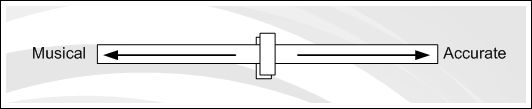
\includegraphics[scale=1.5]{slider1}
\caption{A sliding scale to show how as musicality increases, ability to accurately predict the account's health decreases. The reverse is also true.}
\label{fig:slider1}
\end{figure}

If we also take into account issues of listening fatigue, we may also conclude that the more concentration is required to analyse the music, the harder it is to predict the account's health \textit{(figure \ref{fig:slider2})}. Therefore, the maximum length of a musical sequence will be limited to under 20 seconds.

\begin{figure}[ht]
\centering
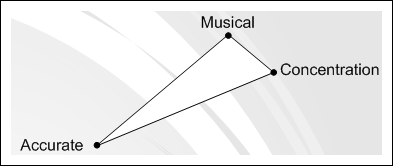
\includegraphics[scale=1.5]{slider2}
\caption{The triangle shows how increasing musicality or an increase in the need for concentration makes it more difficult to accurately predict the account.}
\label{fig:slider2}
\end{figure}


\section{Summary}

In this chapter, we have looked at L-Systems as a way of generating music from accounts. The emergent nature of L-Systems makes them well suited to an application such as music generation.

We have also seen some techniques for generating the L-System from an account, and we have settled on a way to dynamically generate the axiom using a grading system.

Finally, we also formed a hypothesis that the more complex the music, the harder it will be to determine the true nature of the account. As we will soon see, the results of the evaluation will yield some surprises.

In the next chapter, we will fully evaluate this implementation, along with the Signal Mapping approach of the previous chapter.